\chapter{Beispiele/Anwendung}
\section{Einfache Beispiele}
\subsection{erstes}
\[
  P_a=t^2\partial_t^2+t\partial_t+(t^2-n^2)=\sum_{k=0}^2\sum_{l=0}^2
  \alpha_{kl}t^l\partial_t^k
\]

Mit: $\alpha_{2,2}=1$, $\alpha_{1,1}=1$, $\alpha_{0,2}=t^2$ und
$\alpha_{0,0}=n^2$

$
P_a=t^2\partial_t^2+t\partial_t+(t^2-n^2) \Rightarrow 
\begin{cases}
  k=2,l=2 & \Rightarrow u\leq k=2, v\geq l-k=0\\
  k=1,l=1 & \Rightarrow u\leq 1, v\geq 0\\
  k=0,l=0 & \Rightarrow u\leq 0, v\geq 0\\
  k=0,l=2 & \Rightarrow u\leq 0, v\geq 2\\
\end{cases}
$

\begin{center}
  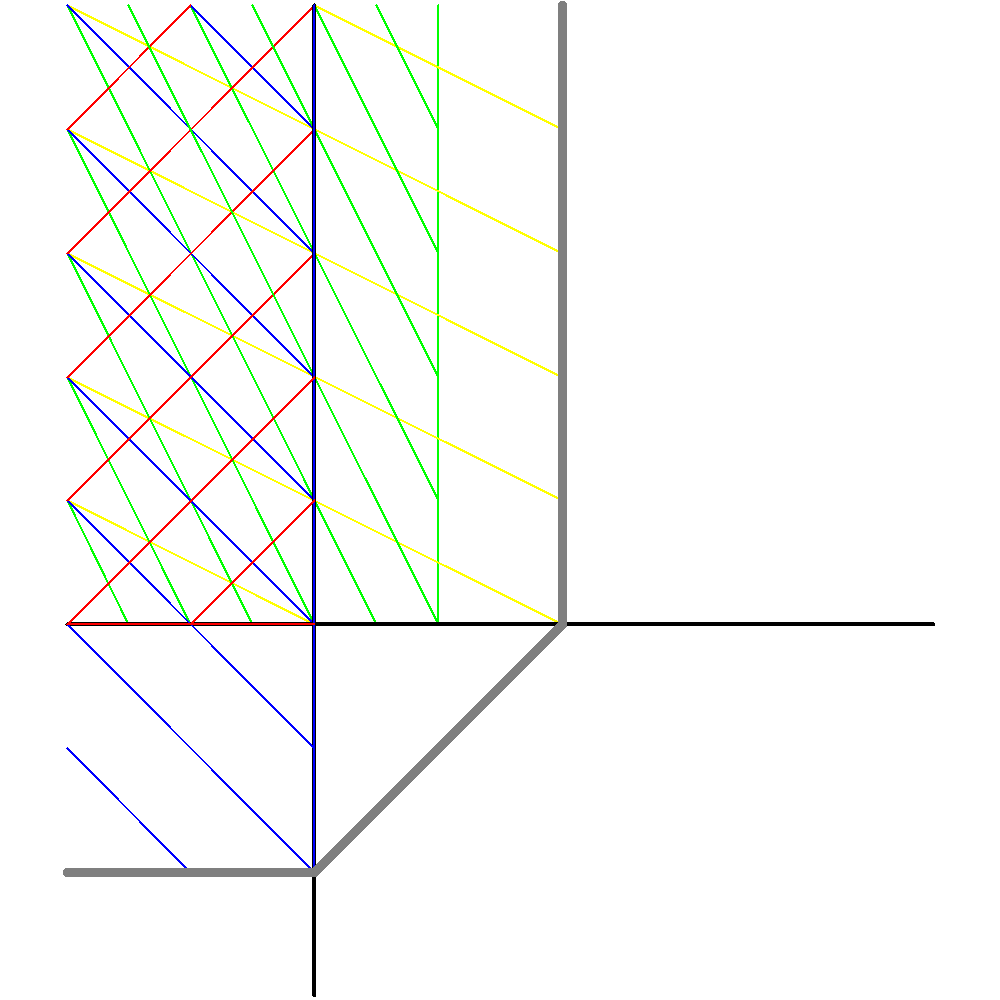
\includegraphics[width=6cm]{beispiele/img/a.png}
\end{center}
also $\slopes(P_a)=\{0\}$ also ist $P_a$ regulär singulär

% vim: set ft=tex :

\subsection{zweites}
\[
  P_b=t\partial_t^2+2\partial_t-1
\]

$
P_b=t\partial_t^2+2\partial_t-1 \Rightarrow 
\begin{cases}
  k=2,l=1 & \Rightarrow u\leq l=2, v\geq l-k=-1\\
  k=1,l=0 & \Rightarrow u\leq 1, v\geq -1\\
  k=0,l=0 & \Rightarrow u\leq 0, v\geq 0\\
\end{cases}
$

\begin{center}
  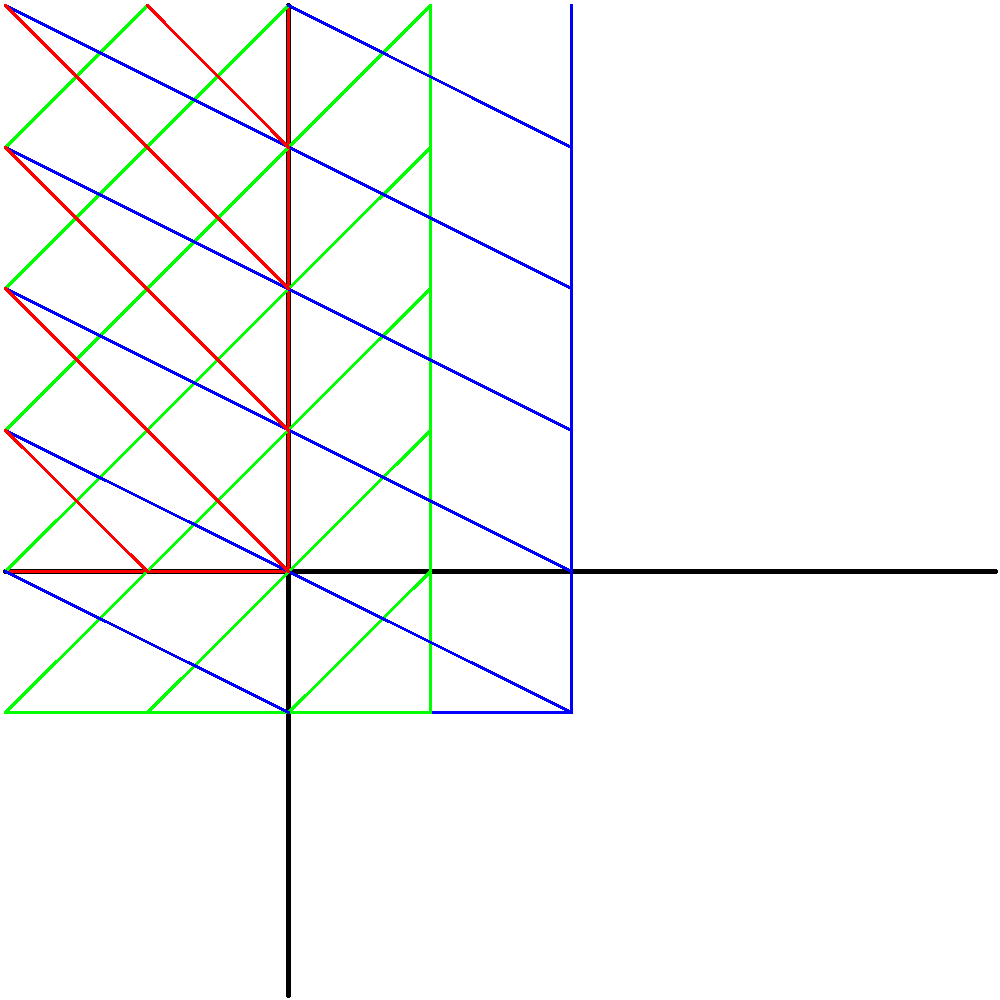
\includegraphics[width=6cm]{beispiele/img/b.png}
\end{center}
also $\slopes(P_b)=\{0\}$ also ist $P_b$ regulär singulär

% vim: set ft=tex :

\subsection{drittes}

\begin{comment}
  zula Barbara Seite 46
\end{comment}


\[
  P_c=t^2\partial_t+1
\]
$
P_c=t^2\partial_t+1
\Rightarrow
\begin{cases}
  k=1, l=2 & \Rightarrow u \leq 1, v \geq 1\\
  k=0, l=1 & \Rightarrow u \leq 0  v \geq 0\\
\end{cases}
$
\begin{center}
  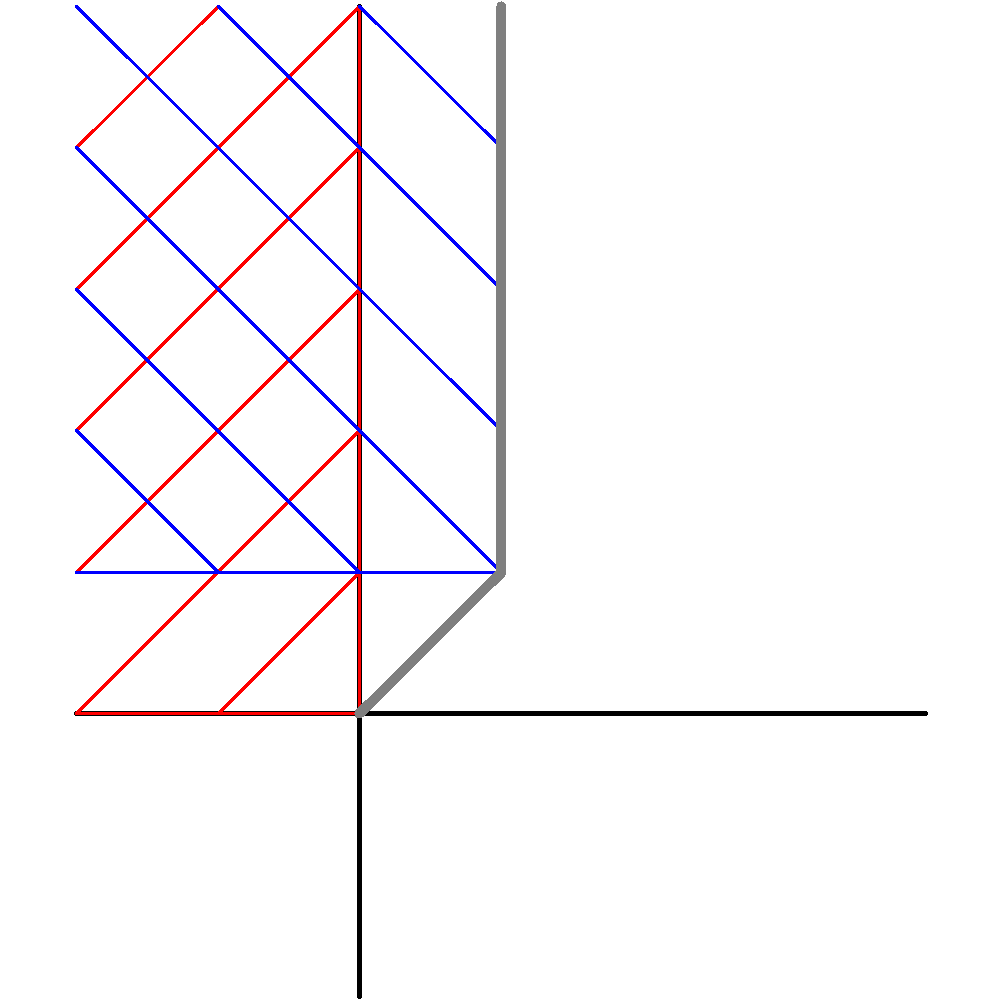
\includegraphics[width=6cm]{beispiele/img/c.png}
\end{center}

also $\slopes(P_c)=\{1\}$.

% vim:set ft=tex :

\subsection{viertes}

\begin{comment}
  zula Barbara Seite 46
\end{comment}

\begin{comment}
  Original aus der Zula:
  \[
    P_d=-3t^{14}\partial_t^6+t^{11}(t+3)\partial_t^5 + 2t^8\partial_t^4
    -t^6(t^3+1)\partial_t^3 + t^4\partial_t
  \]

  $ P_d \Rightarrow
  \begin{cases}
    k=6,l=14 & \Rightarrow u\leq k=6, v\geq l-k=8\\
    k=5,l=12 & \Rightarrow u\leq 5, v\geq 7\\
    k=5,l=11 & \Rightarrow u\leq 5, v\geq 6\\
    k=4,l=8 & \Rightarrow u\leq 4, v\geq 4\\
    k=3,l=9 & \Rightarrow u\leq 3, v\geq 6\\
    k=3,l=6 & \Rightarrow u\leq 3, v\geq 3\\
    k=1,l=4 & \Rightarrow u\leq 1, v\geq 3\\
  \end{cases} $

  also ist Abbildung 5.8 auf seite 53 der zula falsch?
\end{comment}

\[
  P_d=-3t^{14}\partial_t^6+t^{11}(t+3)\partial_t^5 + 2t^8\partial_t^4
  -t^6(t^3+1)\partial_t^3 + t^3\partial_t
\]

$ P_d \Rightarrow
\begin{cases}
  k=6,l=14 & \Rightarrow u\leq k=6, v\geq l-k=8\\
  k=5,l=12 & \Rightarrow u\leq 5, v\geq 7\\
  k=5,l=11 & \Rightarrow u\leq 5, v\geq 6\\
  k=4,l=8 & \Rightarrow u\leq 4, v\geq 4\\
  k=3,l=9 & \Rightarrow u\leq 3, v\geq 6\\
  k=3,l=6 & \Rightarrow u\leq 3, v\geq 3\\
  k=1,l=3 & \Rightarrow u\leq 1, v\geq 2\\
\end{cases} $

\begin{center}
  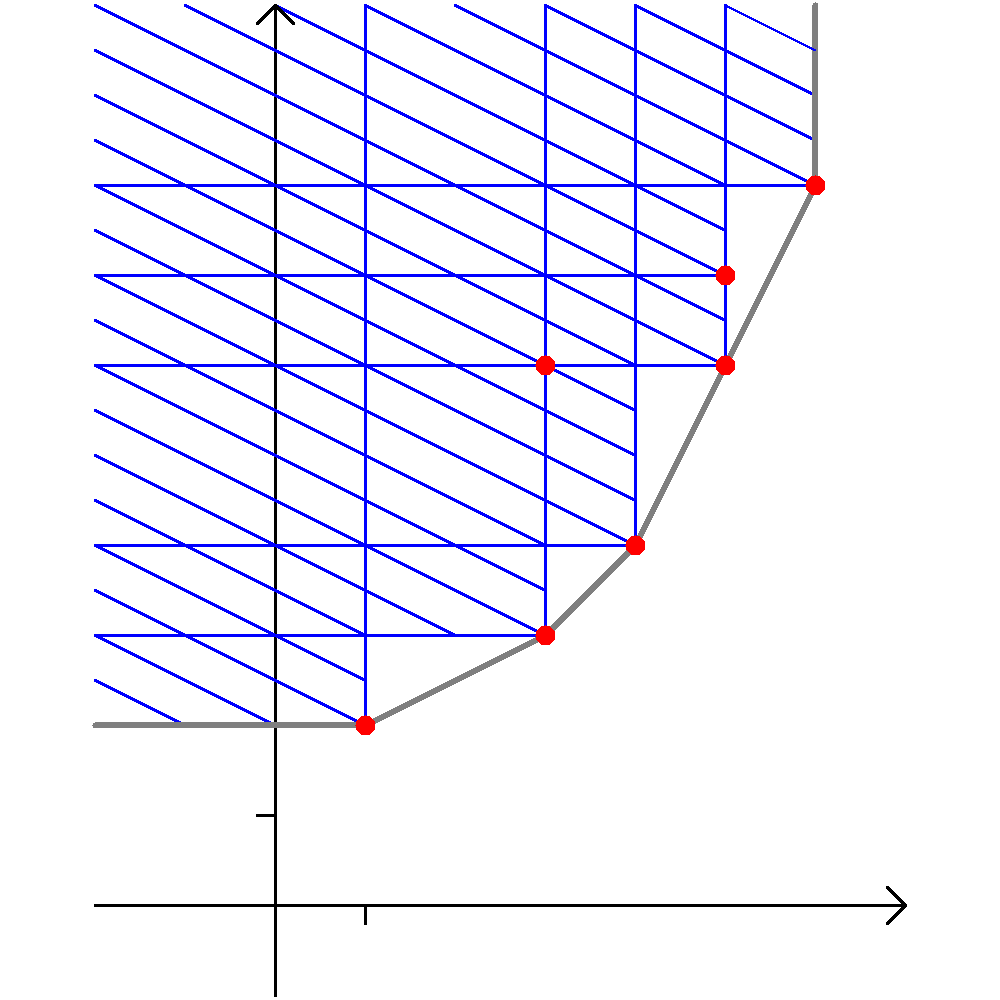
\includegraphics[width=6cm]{beispiele/img/d.png}
\end{center}
also $\slopes(P_b)=\{0,\frac{1}{2},1,2\}$ also ist $P_d$ irregulär singulär.\\
Offenbar ist der Hauptnenner der Steigugnen gleich $2$.\\
Betrachte also $\rho:t\mapsto u^2$\\
und erhalte: ???

% vim: set ft=tex :

\subsection{bsp e}

\[
  P_e=t^4(t+1)\partial_t^4 + t\partial_t^2+\frac{1}{t}\partial_t+1
\]

\begin{center}
  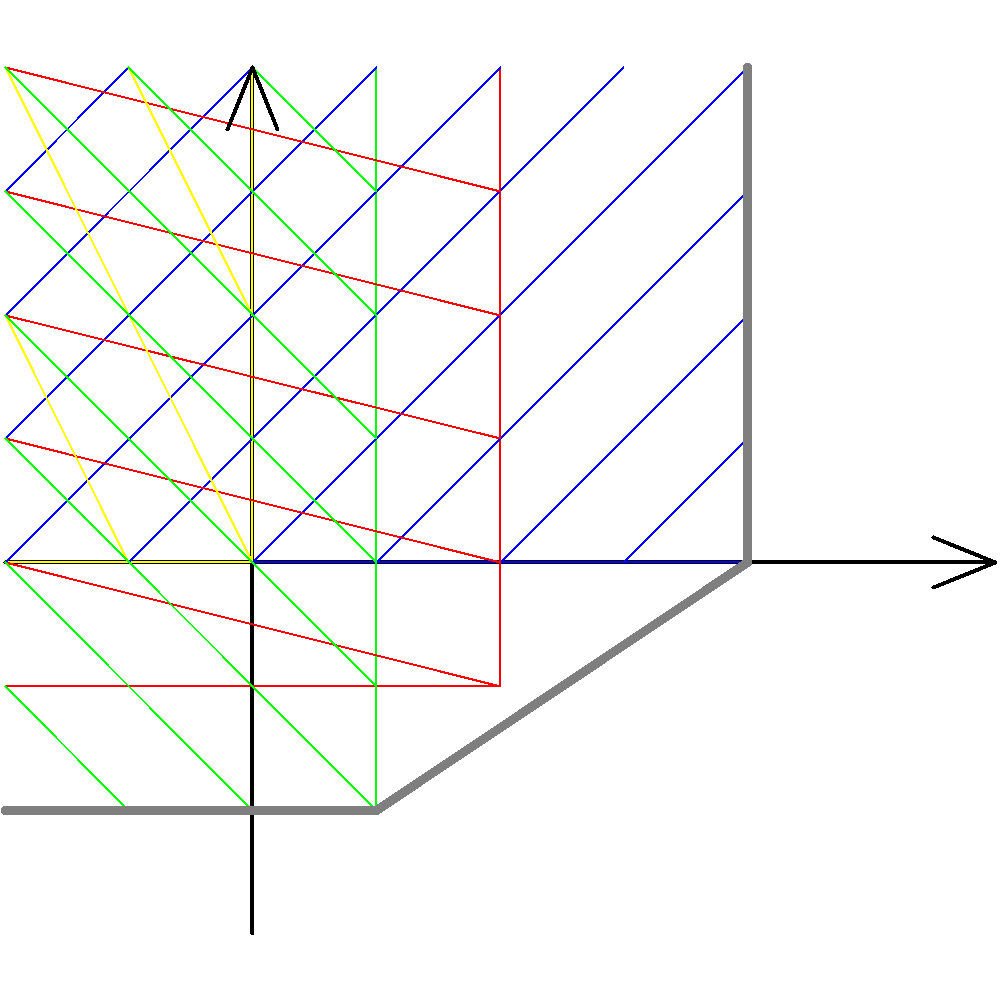
\includegraphics[width=6cm]{beispiele/img/e.png}
\end{center}

also $\slopes(P_e)=\{0,\frac{2}{3}\}$

Dies gilt Analog für das einfachere:
\[
  \bar P_e=t^4\partial_t^4 +\frac{1}{t}\partial_t
\]

\begin{center}
  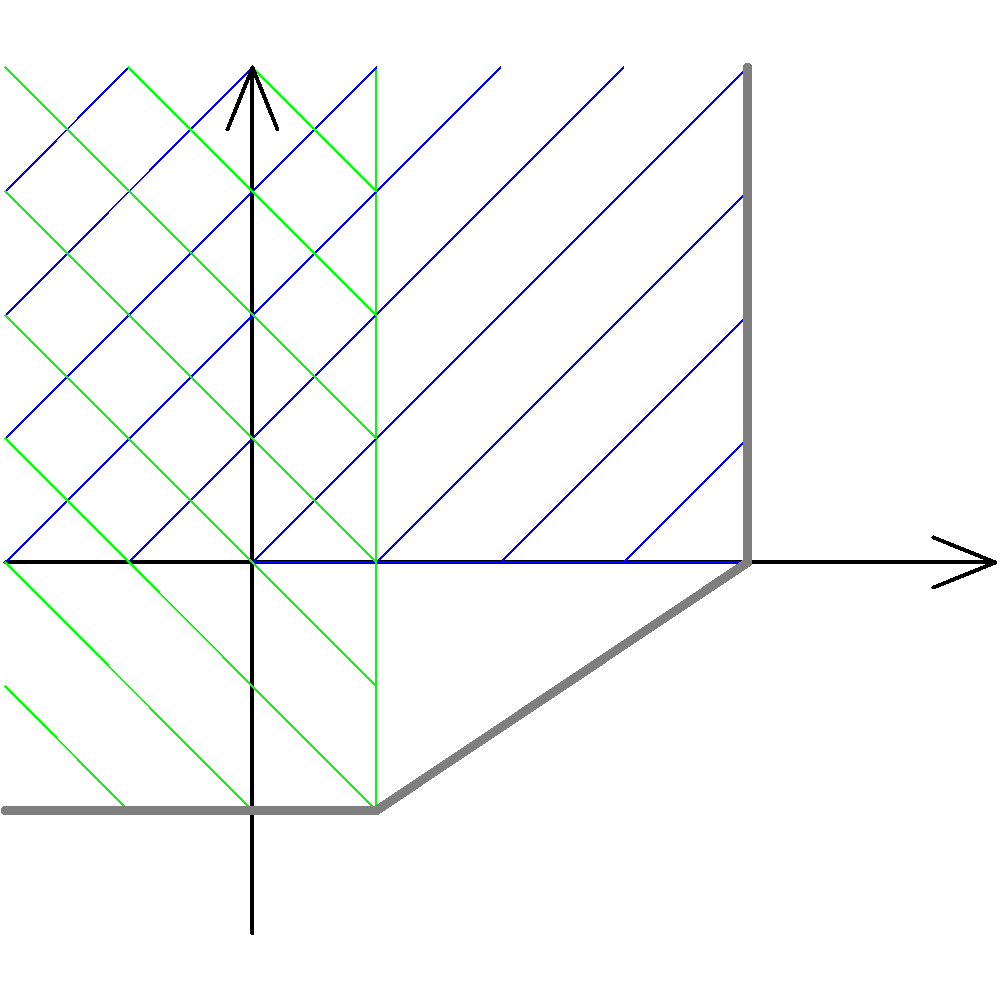
\includegraphics[width=6cm]{beispiele/img/bar_e.png}
\end{center}

% vim: set ft=tex :

\begin{comment}
  \[
    Sabbah\_Fourier-local.pdf \rightarrow 5.b.
  \]
\end{comment}
\section{Meromorpher Zusammenhang der formal, aber nicht Konvergent, zuerfällt}
\begin{comment}
  Quellen??
  \[
    \sum n!x^n
  \]
\end{comment}

% vim: set ft=tex :
